\documentclass[10pt]{article}
\usepackage[utf8]{inputenc}
\usepackage[T1]{fontenc}
\usepackage{amsmath}
\usepackage{amsfonts}
\usepackage{amssymb}
\usepackage[version=4]{mhchem}
\usepackage{stmaryrd}
\usepackage{hyperref}
\usepackage{graphicx}
\usepackage{enumitem}
\usepackage{multirow}
\usepackage{amsthm}
\graphicspath{ {./CS-234/} }

\title{Midterm 2 Prep}

\author{CS 234}
\date{Daniel Lee}


\begin{document}
\maketitle

\section*{1 \quad Midterm 2 Prep}

\begin{enumerate}[label={}]
    \item 7.2 Show that if $x$ and $y$ are odd length strings and $z$ is an even length string that $x y z$ is an even length string.\\

    \item 7.8 Show that for all $n \geq 3,4 n^2+6 n \leq 2 n^3$.\\

    \item 7.10 Define the $N O R$ operation as $\operatorname{NOR}\left(L_1, L_2\right)=\left\{x: x \notin L_1 \wedge x \notin L_2\right\}$. Show that regular languages are closed under the $N O R$ operator.\\

    \item Prove the following by giving constants and then showing that the inequalities hold:

          D.4 $2 n^2+4 n=O\left(n^2\right)$\\

          D.5 $3 n^2-4 n+5=O\left(n^2\right)$\\

          D.9 $4 n^2-3 n=\Omega\left(n^2\right)$\\

          D.10 $n^2-2 n+3=\Omega\left(n^2\right)$\\

          D.13 $n+8=\Theta(n)$\\

          D.14 $n^2+2 n=\Theta\left(n^2\right)$\\

          D.16 $n^2=o\left(n^3\right)$\\

          D.17 $100 n^3=o\left(n^4\right)$\\

          D.18 $n^5=\omega\left(n^4\right)$\\

          D.19 $10 n^3=\omega\left(n^2\right)$\\

    \item Prove the following using induction:\\

          8.5 Show that $\sum_{i=1}^n \frac{1}{i(i+1)}=\frac{n}{n+1}$ for all $n \geq 1$.\\

          8.12 Write a recursive function to find the minimum of a list and show that it is correct.\\

          8.29 Show that it is possible to use postage stamps of values 3 and 5 to make any amount of postage $n \geq 8$.\\


          The $n^{\text {th }}$ Fibonacci number is given by $F(n)$, which is defined by the following recursive recurrence equation:

          $$
              F(n)= \begin{cases}0 & n=0 \\ 1 & n=1 \\ F(n-1)+F(n-2) & n \geq 2\end{cases}
          $$


          For this task, show that $F(n+1) \geq 1.5 \cdot F(n)$ for all $n \geq 2$.\\


    \item Draw DFAs with as few states as possible for each of the following languages and then prove that they accept that language.\\

          9.3 $\left\{w \in\{0,1\}^*: w\right.$ has 01 as a substring $\}$\\

          9.12 $\left\{w \in\{0,1\}^*: w\right.$ has exactly one 0$\}$\\

          \newpage

    \item 7.2 Show that if $x$ and $y$ are odd length strings and $z$ is an even length string that $x y z$ is an even length string.

          Let $x$ and $y$ be odd length of strings and $z$ be an even length string.\\
          WTS that xyz is an even length of string.\\
          By the def. 7.2 in the text book, we know that there exist some integers p, q $\geq$ 0 such that $|x|=2 p+1,|y|=2 q+1$.\\
          Also, by the def. 7.1 in the text book, we know that there exists some integer r $\geq$ 0 such that $|z|=2 r$.\\
          Then, the length of the string $x y z$ is the sum of the lengths of $x, y$, and $z$, or $2 p+1+2 q+1+2 r=2(p+q+r+1)$. [def. 7.1]\\
          Since we can write the length of $x y z$ as $2s$ (where $s=p+q+r+1 \geq 0$ is an integer), this means that it follows by def 7.1 that $x y z$ is an even length string. $Q.E.D.$\\


    \item 7.8 Show that for all $n \geq 3,4 n^2+6 n \leq 2 n^3$.

          Let us assume that $n \geq 3$. Then we can write
          $$
              \begin{aligned}
                  4 n^2+6 n & \leq 4 n^2+2 n^2
                            & {\left[\text { as } 6 n \leq 2 n^2 \text { since } 3 \leq n\right] } \\
                            & = 6 n^2 \quad[\text { math }]                                        \\
                            & \leq 2 n^3 \quad[\text { as } 3 \leq n],
              \end{aligned}
          $$

          which shows that $4 n^2+6 n \leq 2 n^3$.
          Thus, $4 n^2+6 n$ is at most $2 n^3$ for all $n \geq 3$. $Q.E.D.$\\

    \item 7.10 Define the $N O R$ operation as $\operatorname{NOR}\left(L_1, L_2\right)=\left\{x: x \notin L_1 \wedge x \notin L_2\right\}$. Show that regular languages are closed under the $N O R$ operator.

          Suppose $L_1$ and $L_2$ are regular languages.\\
          WTS $\operatorname{NOR}\left(L_1, L_2\right)=\left\{x: x \notin L_1 \wedge x \notin L_2\right\}$ is regular.\\
          By the proof of theorem which was demonstrated in class that regular languages are closed under union, we know that
          $\left\{x: x \in L_1\right\} \cup \left\{x:x \in L_2\right\} = \left\{x: x \in L_1 \vee x \in L_2\right\}$ is regular.\\
          Also by the proof of theorem which was demonstrated in class that regular languages are closed under complement, we know that $\left\{x: x \in L_1 \vee x \in L_2\right\}^c = \left\{x: x \notin L_1 \wedge x \notin L_2\right\}$ is regular. \quad[\text { De Morgan's laws }]\\
          Thus, regular languages are closed under the $N O R$ operator by the theorems above. $Q.E.D.$

    \item Prove the following by giving constants and then showing that the inequalities hold:


          D.4 $2 n^2+4 n=O\left(n^2\right)$
          \begin{proof}
              Let $n$ be an arbitrary real number that is at least 4.\\
              Then the following inequality holds:
              $$
                  \begin{aligned}
                      2n^2+4n & \leq 2 n^2+ n^2
                              & {\left[n \geq 4\right] } \\
                              & = 3 n^2 .
                  \end{aligned}
              $$
              Thus $2 n^2+4n \leq 3 n^2$, so picking $n_0=4$ and $c=3$ witnesses \\$\exists n_0, c>0 .\quad \forall n \geq n_0 .\quad 2 n^2+4n \leq c \cdot n^2$.\\
                  Thus, by the definition of big-O, $2 n^2+4n \in O\left(n^2\right)$.\\
          \end{proof}
          D.5 $3 n^2-4 n+5=O\left(n^2\right)$
          \begin{proof}
              Let $n$ be an arbitrary real number that is at least 1.\\
              Then the following inequality holds:
              $$
                  \begin{aligned}
                      3n^2-4n+5 & \leq 3n^2+n^2+5n^2
                                & {\left[\text { as } -4n \leq n^2 \text { and } 5 \leq 5n^2 \text { for all } n \geq 1\right] } \\
                                & = 9 n^2 .
                  \end{aligned}
              $$
              Thus $3 n^2-4 n+5 \leq 9 n^2$, so picking $n_0=1$ and $c=9$ witnesses \\$\exists n_0, c>0 .\quad \forall n \geq n_0 .\quad 3 n^2-4 n+5 \leq c \cdot n^2$.\\
                  Thus, by the definition of big-O, $3 n^2-4 n+5 \in O\left(n^2\right)$.\\
          \end{proof}
          \newpage

          D.9 $4 n^2-3 n=\Omega\left(n^2\right)$
          \begin{proof}
              Let $n$ be an arbitrary real number that is at least 1 and let $c$ be 1.\\
              We want to show that there exists $n_0, c > 0$ such that for all $n\geq n_0$ we have that $4 n^2-3 n\geq c \cdot n^2$.\\
              Observe the following inequality:\\
              $$
                  \begin{aligned}
                      4 n^2-3 n=n(4 n-3) & \geq c \cdot n \cdot n = n^2 \quad[c=1]. \\
                  \end{aligned}
              $$

              Since we initially assumed that $n$ is an arbitrary real number that is at least 1, we know by arithmetic that
              $$
                  \begin{aligned}
                      4 n-3 & \geq n \quad[\text { math }].
                  \end{aligned}
              $$
              Therefore,
              $$
                  \begin{aligned}
                      3 (n-1) & \geq 0 \quad[\text { math }]. \\
                  \end{aligned}
              $$

              Thus picking $n_0=1$ and $c=1$ witnesses \\$\exists n_0, c>0 .\quad \forall n \geq n_0 .\quad 4 n^2-3 n \geq c \cdot n^2$.\\
                  Thus, by the definition of big-$\Omega$, $4 n^2-3 n \in \Omega\left(n^2\right)$.\\
          \end{proof}
          D.10 $n^2-2 n+3=\Omega\left(n^2\right)$
          \begin{proof}
              Let $n$ be an arbitrary real number that is at least 1 and let $c$ be $\frac{1}{2}$.\\
              We want to show that there exists $n_0, c > 0$ such that for all $n\geq n_0$ we have that $n^2-2 n+3 \geq c \cdot n^2$.\\
              Observe the following inequality:\\
              $$
                  \begin{aligned}
                       & n^2-2 n+3 \geq c \cdot n \cdot n =\frac{1}{2} \cdot n^2 \quad\left[c=\frac{1}{2}\right].
                  \end{aligned}
              $$
              Therefore, by arithmetics, we know that
              $$
                  \begin{aligned}
                       & \frac{1}{2} n^2-2 n+3 \geq 0 \quad[\text { math }].
                  \end{aligned}
              $$
              We can rewrite the above mathematical expression as
              $$
                  \begin{aligned}
                       & \frac{1}{2}\left(n^2-4 n\right)+3 \geq 0 \quad[\text { math }].
                  \end{aligned}
              $$
              Therefore, by arithmetics, we know that
              $$
                  \begin{aligned}
                       & \frac{1}{2}(n-2)^2-2+3=\frac{1}{2}(n-2)^2+1 \geq 0 \quad[\text { math }].
                  \end{aligned}
              $$

              Thus picking $n_0=1$ and $c=\frac{1}{2}$ witnesses \\$\exists n_0, c>0 .\quad \forall n \geq n_0 .\quad n^2-2 n+3 \geq c \cdot n^2$.\\
                  Thus, by the definition of big-$\Omega$, $n^2-2 n+3 \in \Omega\left(n^2\right)$.\\
          \end{proof}
          \newpage

          D.13 $n+8=\Theta(n)$
          \begin{proof}
              To show this, by definition of big-$\Theta$, it suffices to show $n+8 \in O\left(n\right)$ and $n+8 \in \Omega\left(n\right)$.\\
              Let $n$ be an arbitrary real number that is at least 1.\\
              Then the following inequality holds:
              $$
                  \begin{aligned}
                      n+8 & \leq n+8n
                          & {\left[n \geq 1\right] } \\
                          & = 9n .
                  \end{aligned}
              $$
              Thus $n+8 \leq 9n$, so picking $n_0=1$ and $c_1=9$ witnesses \\$\exists n_0, c_1>0 .\quad \forall n \geq n_0 .\quad n+8 \leq c_1 \cdot n$.\\
                  Thus, by the definition of big-O, $n+8 \in O\left(n\right)$.\\
                  Also, let $n$ be an arbitrary real number that is at least 1 and let $c_2$ be 1. Observe the following inequality:
                  $$
                      \begin{aligned}
                          n+8 & \geq n
                              & {\left[n \geq 1\right] }. \\
                      \end{aligned}
                  $$
                  Thus picking $n_0=1$ and $c_2=1$ witnesses \\$\exists n_0, c_2>0 .\quad \forall n \geq n_0 .\quad n+8 \geq c_2 \cdot n$.\\
                  Thus, by the definition of big-$\Omega$, $n+8 \in \Omega\left(n\right)$.\\
                  Finally, because both $n+8 \in O\left(n\right)$ and $n+8 \in \Omega\left(n\right)$, it follows that $n+8\in\Theta(n)$ by definition.\\
          \end{proof}

          D.14 $n^2+2 n=\Theta\left(n^2\right)$
          \begin{proof}
              To show this, by definition of big-$\Theta$, it suffices to show $n^2+2n \in O\left(n^2\right)$ and $n^2+2n \in \Omega\left(n^2\right)$.\\
              Let $n$ be an arbitrary real number that is at least 1.\\
              Then the following inequality holds:
              $$
                  \begin{aligned}
                      n^2+2 n & \leq n^2+2 n^2
                              & {\left[n \geq 1\right] } \\
                              & = 3n^2 .
                  \end{aligned}
              $$
              Thus $n^2+2 n \leq 3n^2$, so picking $n_0=1$ and $c_1=3$ witnesses \\$\exists n_0, c_1>0 .\quad \forall n \geq n_0 .\quad n^2+2 n \leq c_1 \cdot n^2$.\\
                  Thus, by the definition of big-O, $n^2+2 n \in O\left(n^2\right)$.\\
                  Also, let $n$ be an arbitrary real number that is at least 1 and let $c_2$ be 1. Observe the following inequalities:
                  $$
                      \begin{aligned}
                          n^2+2 n & \geq n^2
                                  & {\left[n \geq 1\right] }. \\
                      \end{aligned}
                  $$
                  By arithmetic, we know that
                  $$
                      \begin{aligned}
                           & 2n \geq 0 \quad [\text { math }]. \\
                      \end{aligned}
                  $$
                  Thus picking $n_0=1$ and $c_2=1$ witnesses \\$\exists n_0, c_2>0 .\quad \forall n \geq n_0 .\quad n^2+2 n \geq c_2 \cdot n^2$.\\
                  Thus, by the definition of big-$\Omega$, $n^2+2 n \in \Omega\left(n^2\right)$.\\
                  Finally, because both $n^2+2 n \in O\left(n^2\right)$ and $n^2+2 n \in \Omega\left(n^2\right)$, it follows that $n^2+2 n\in\Theta(n^2)$ by definition.\\
          \end{proof}

          \newpage

          D.16 $n^2=o\left(n^3\right)$
          \begin{proof}
              Let $c$ be an arbitrary positive real number.\\
              Then let $n$ be an arbitrary real number that is strictly greater than $\frac{1}{c}$. Observe the following inequalities that they hold.\\
              $$
                  \begin{aligned}
                      c \cdot n^3 & >c \cdot \frac{1}{c} \cdot n^2 &  & {\left[n>\frac{1}{c}\right] } \\
                                  & =n^2                           &  & {[\text { math }]. }
                  \end{aligned}
              $$

              Thus picking an arbitrary positive real number $n_0$ to be strictly greater than $\frac{1}{c}$ witnesses that $\forall c>0 . \quad \exists n_0>0 . \quad \forall n \geq n_0 . \quad$ $n^2$ $< c \cdot n^3$. By the definition of little-$o$, this means that $n^2 \in o\left(n^3\right)$.\\
          \end{proof}
          D.17 $100 n^3=o\left(n^4\right)$
          \begin{proof}
              Let $c$ be an arbitrary positive real number.\\
              Then let $n$ be an arbitrary real number that is strictly greater than $\frac{100}{c}$. Observe the following inequalities that they hold.\\
              $$
                  \begin{aligned}
                      c \cdot n^4 & >c \cdot \frac{100}{c} \cdot n^3 &  & {\left[n>\frac{100}{c}\right] } \\
                                  & =100n^3                          &  & {[\text { math }]. }
                  \end{aligned}
              $$

              Thus picking an arbitrary positive real number $n_0$ to be strictly greater than $\frac{100}{c}$ witnesses that $\forall c>0 . \quad \exists n_0>0 . \quad \forall n \geq n_0 . \quad$ $100 n^3$ $< c \cdot n^4$. By the definition of little-$o$, this means that $100n^3 \in o\left(n^4\right)$.\\
          \end{proof}
          D.18 $n^5=\omega\left(n^4\right)$
          \begin{proof}
              Let $c$ be an arbitrary positive real number. Then let $n$ be an arbitrary real number that is strictly greater than $c$.
              We want to show that for all $c>0$, there exists a constant $n_0 > 0$ such that for all $n\geq n_0$, $n^5>c \cdot n^4$.
              Observe the following inequalities that they hold.
              $$
                  \begin{aligned}
                      n^5                   & >c \cdot n^4 \quad {\left[n>c>0\right] } \\
                      \longleftrightarrow n & >c \quad[\text { math }].
                  \end{aligned}
              $$
              We earlier assumed that $n>c$ so we can observe that for all $n\geq n_0$, $n\geq n_0>c$.
              Thus picking $n_0$ to be strictly greater than $c$ witnesses that $\forall c>0$. $\exists n_0>0$. $\forall n \geq n_0$. $n^5>c \cdot n^4$.\\
              By the definition of little-$\omega$, it follows that $n^5 \in \omega\left(n^4\right)$.\\
          \end{proof}
          \newpage

          D.19 $10 n^3=\omega\left(n^2\right)$
          \begin{proof}
              Let $c$ be an arbitrary positive real number.
              Then let $n$ be an arbitrary real number that is strictly greater than $\frac{c}{10}$.
              We want to show that for all $c>0$, there exists a constant $n_0 > 0$ such that for all $n\geq n_0$, $10 n^3>c \cdot n^2$.
              Observe the following inequalities that they hold.
              $$
                  \begin{aligned}
                      10 n^3                & >c \cdot n^2 \quad {\left[n>\frac{c}{10}>0\right] } \\
                      \longleftrightarrow n & >\frac{c}{10} \quad[\text { math }].
                  \end{aligned}
              $$
              We earlier assumed that $n>\frac{c}{10}$ so we can observe that for all $n\geq n_0$, $n\geq n_0>\frac{c}{10}$.
              Thus picking $n_0$ to be strictly greater than $\frac{c}{10}$ witnesses that $\forall c>0$. $\exists n_0>0$. $\forall n \geq n_0$. $10 n^3>c \cdot n^2$.\\
              By the definition of little-$\omega$, it follows that $10 n^3 \in \omega\left(n^2\right)$.\\
          \end{proof}

    \item Prove the following using induction:\\

          8.5 Show that $\sum_{i=1}^n \frac{1}{i(i+1)}=\frac{n}{n+1}$ for all $n \geq 1$.
          \begin{proof}
              The statement can be proven by induction, letting the inductive predicate $P(n)$ be defined as $\sum_{i=1}^n \frac{1}{i(i+1)}=\frac{n}{n+1}$.\\

              \textbf{Base case} $n=1$: For the base case, when $n=1$, the sum shows that $\sum_{i=1}^1 \frac{1}{i(i+1)}=\frac{1}{1\cdot2}=\frac{1}{2}$. The formula $\frac{n}{n + 1}=\frac{1}{1+1}$ is also equal to $\frac{1}{2}$. Hence the base case $P(1)$ holds.\\

              \textbf{Inductive case :} Suppose for the inductive hypothesis that $P(k)$ holds for an arbitray $k \geq 1$. That is, suppose $\sum_{i=1}^k \frac{1}{i(i+1)}=\frac{k}{k+1}$.
              We then want to show that $P(k+1)$ holds. That is, we want to show that $\sum_{i=1}^{k+1} \frac{1}{i(i+1)}=\frac{k+1}{k+1+1}=\frac{k+1}{k+2}$.\\
              To show this statement, we use the following chain of equalities:
              $$
                  \begin{aligned} \sum_{i=1}^{k+1} \frac{1}{i(i+1)} & =\left(\sum_{i=1}^k \frac{1}{i(i+1)}\right)+\frac{1}{(k+1)(k+2)} & {\left[\sum \text { def}\right] } \\ & =\frac{k}{k+1}+\frac{1}{(k+1)(k+2)} & {\left[\text {I H}\right] }\\ & =\frac{k(k+2)+1}{(k+1)(k+2)} & {\left[\text {algebra}\right] }\\ & =\frac{k^2+2 k+1}{(k+1)(k+2)} & {\left[\text {algebra}\right] } \\ & =\frac{(k+1)^2}{(k+1)(k+2)} & {\left[\text {algebra}\right] } \\ & =\frac{k+1}{k+2} & {\left[\text {algebra}\right] }.
                  \end{aligned}
              $$

              Thus $P(k+1)$ holds.\\

              \textbf{Conclusion:} Because both the base case and inductive case hold, induction allows us to conclude $\sum_{i=1}^n \frac{1}{i(i+1)}=\frac{n}{n+1}$ for all $n \geq 1$.
          \end{proof}

          8.12 Write a recursive function to find the minimum of a list and show that it is correct.\\

          input: A list of integers of length at least 1.\\
          output: A minimum of the given list.\\
          1. def $\operatorname{minList}(\text{intList})$:\\
          2. \quad if len(intList) == 1:\\
          3. \quad \quad return intList[0]\\
          4. \quad endElt $= \text {intList.}\operatorname{pop}()$\\
          5. \quad minVal = minList(intList)\\
          6. \quad if minVal < endElt:\\
          7. \quad \quad return minVal\\
          8. \quad else:\\
          9. \quad \quad return endElt\\

          \begin{proof}

              The proof of the recursive function minList(intList) follows by induction over a given list. For this purpose, let $P(l)$ be the inductive predicate that the minimum of the list $l$ is minList$(l)$. We now show both the base case and inductive case.

              \textbf{Base case} len($l$) = 1: Note that the length of the list should be at least 1. For the list $l_1$ where its length is 1, we know that there is only one element in the list, which is of course the only one element would be the minimum of the given list. And because the length of the list $l_1$ is 1, the conditional statement in the $\# 2$ codeline of minList(intList) will be true, so minList $\left(l_1\right)$ will return the only one element in the list by \#3 codeline. Thus $P\left(l_1\right)$ where $l_1$ is the list with its length is 1 holds.

              \textbf{Inductive case :} For the inductive hypothesis, assume $P\left(l_2\right)$ holds for an arbitrary list $l_2$ of length $n \geq 1$. We want to show that an arbitrary list $l_3$ of length $n+1$ also holds by returning the minimum of the list $l_3$. Because by $\# 4$ codeline where it would extract the last element in list $l_3$, the length of list $l_3$ will turn into $n$, which is the same length with $l_2$. And by the inductive hypothesis, we know that with $\# 5$ codeline being run, the minimum of list $l_3$, which its length was reduced to $n$, will be correctly saved in the minVal variable.
              We now proceed by cases on whether minVal < endElt:

              \textbf{Subcase }minVal < endElt: Suppose minVal < endElt. Then we know that this means the minimum of the list $l_3$, which its length was reduced to $n$, is less than the extracted element endElt. Therefore, we witness that minVal is the minimum of the original list $l_3$ with its length $n+1$. The conditional statement in \#6 codeline will be true and therefore the minList(intList) function returns minVal by running the \#7 codeline. Thus $P\left(l_3\right)$ where $l_3$ is the list with its length $n+1$ holds.


              \textbf{Subcase }minVal $\geq$ endElt: Suppose minVal $\geq$ endElt. Then we know that this means the extracted element endElt is less than or equal to the minimum of the list $l_3$, which its length was reduced to $n$. Therefore, we witness that endElt is the minimum of the original list $l_3$ with its length $n+1$. The conditional statement in \#6 codeline will be false, which makes the \#8 codeline being run and the minList(intList) function returns endElt by running the \#9 codeline. Thus $P\left(l_3\right)$ where $l_3$ is the list with its length $n+1$ also holds in this case too.

              \textbf{Conclusion:} Because both the base case and inductive case hold, induction allows us to conclude that for all lists of length n $\geq$ 1, the minimum of the list $l$ is minList$(l)$.

          \end{proof}

          8.29 Show that it is possible to use postage stamps of values 3 and 5 to make any amount of postage $n \geq 8$.
          \begin{proof}
              The statement can be proven by strong induction, letting the inductive predicate $P(n)$ be defined as it is possible to use postage stamps of values 3 and 5 to make any amount of postage $n \geq 8$.

              \textbf{Base case} $n = 8$: To show that $P(8)$ holds, first observe that $8=3+5$. Then observe that it is possible to make 8 amounts of postage by using one postage stamp of value 3 and one postage stamp of value 5. These two observations show that $P(8)$ holds.


              \textbf{Base case} $n = 9$: To show that $P(9)$ holds, first observe that $9=3+3+3$. Then observe that it is possible to make 9 amounts of postage by using three postage stamps of value 3. These two observations show that $P(9)$ holds.


              \textbf{Base case} $n = 10$: To show that $P(10)$ holds, first observe that $10=5+5$. Then observe that it is possible to make 10 amounts of postage by using two postage stamps of value 5. These two observations show that $P(10)$ holds.

              \textbf{Inductive case :} Assume for the inductive hypothesis that, for some $n \geq 10, P(k)$ holds for all $8 \leq k \leq n$, where $k$ can be expressed with nonnegative integers $x$ and $y$ as follows:

              $$
                  \begin{aligned}
                      k & = 3x +5y.
                  \end{aligned}
              $$

              We now want to show that $P(n+1)$ holds.
              First, we know that $n-2 \geq 8$ since $n \geq 10$ and by the inductive hypothesis, we can express $n-2$ with nonnegative integers $x$ and $y$ as follows:

              $$
                  \begin{aligned}
                      n-2 & = 3x + 5y & [\text { I H }].
                  \end{aligned}
              $$


              Second observe that by using one more postage stamp of value 3 allows us to observe the following equalities:

              $$
                  \begin{aligned}
                      (n-2) + 3 & = n + 1       & [\text { math }]  \\
                                & = 3x + 5y + 3 & [\text { I H }]   \\
                                & =3(x+1) + 5y  & [\text { math }].
                  \end{aligned}
              $$


              We know that $x+1$ and $y$ are nonnegative integers, thus $P(n+1)$ holds.\\

              \textbf{Conclusion:} Thus, by strong induction, we can conclude that it is possible to use postage stamps of values 3 and 5 to make any amount of postage $n \geq 8$.
          \end{proof}



          The $n^{\text {th }}$ Fibonacci number is given by $F(n)$, which is defined by the following recursive recurrence equation:

          $$
              F(n)= \begin{cases}0 & n=0 \\ 1 & n=1 \\ F(n-1)+F(n-2) & n \geq 2\end{cases}
          $$


          For this task, show that $F(n+1) \geq 1.5 \cdot F(n)$ for all $n \geq 2$.

          \begin{proof}
              The statement can be proven by strong induction, letting the indcutive predicate $P(n)$ be defined as $F(n+1) \geq 1.5 \cdot F(n)$.

              \textbf{Base case} $n=2$: For the base case, when $n=2$, observe the following equalities:
              $$
                  \begin{aligned}
                      F(3) & = F(2) + F(1)
                           & {\left[\text {F def}\right] } \\
                           & = F(1) + F(0) + F(1)
                           & {\left[\text {F def}\right] } \\
                           & = 2
                           & {\left[math\right] }.         \\
                  \end{aligned}
              $$
              Now observe the following equalities:
              $$
                  \begin{aligned}
                      F(2) & = F(1) + F(0)
                           & {\left[\text {F def}\right] } \\
                           & = 1
                           & {\left[math\right] }.         \\
                  \end{aligned}
              $$

              We now know that $F(3) = 2$ and $F(2) = 1$, we can witness that $F(3) \geq 1.5 \cdot F(2)$, and so $P(2)$ holds.\\

              \textbf{Base case} $n=3$: For the base case, when $n=3$, observe the following equalities:
              $$
                  \begin{aligned}
                      F(4) & = F(3) + F(2)
                           & {\left[\text {F def}\right] }                        \\
                           & = 3
                           & {\left[\text{as $F(3) = 2$ and $F(2) = 1$}\right] }. \\
                  \end{aligned}
              $$
              We now know that $F(4) = 3$ and $F(3) = 2$, we can witness that $F(4) \geq 1.5 \cdot F(3)$, and so $P(3)$ holds.\\

              \textbf{Inductive case :} Assume for the inductive hypothesis that, for some natural $n \geq 3$, $P(k)$ holds for all $2 \leq k \leq n$. We then want to show that $P(n+1)$ holds, i.e., that $F(n+2) \geq 1.5 \cdot F(n+1)$.\\
              We know that by the given definition of $F(n)$, we can observe the following equality:
              $$
                  \begin{aligned}
                      F(n+2) & =F(n+1)+F(n) & {\left[\text {F def}\right] }. \\
                  \end{aligned}
              $$
              So to show that $P(n+1)$ holds, we need to show the following inequality:
              $$
                  \begin{aligned}
                      F(n+1)+F(n) \geq 1.5 \cdot F(n+1).
                  \end{aligned}
              $$
              By the inductive hypothesis, observe the following inequalities that they hold when $k=n-1$:
              $$
                  \begin{aligned}
                      F(n)                       & \geq 1.5 \cdot F(n-1)                        & {\left[\text {I H}\right] }   \\
                      \longleftrightarrow F(n-1) & \leq \frac{F(n)}{1.5}=\frac{2}{3} \cdot F(n) & {\left[\text {math}\right] }. \\
                  \end{aligned}
              $$
              As we know that $F(n+1)=F(n)+F(n-1)$ by definition, observe the following inequality:
              $$
                  \begin{aligned}
                      F(n+1)=F(n)+F(n-1) & \leq F(n)+\frac{2}{3} \cdot F(n) \quad\left[\text {I H}\right] \\
                                         & =\frac{5}{3} \cdot F(n) \quad[\text { math }] .
                  \end{aligned}
              $$
              We can rewrite the above inequality as
              $$
                  \begin{aligned}
                      F(n) \geq \frac{3}{5} \cdot F(n+1) \quad[\text { math }].
                  \end{aligned}
              $$
              Now, observe the following inequality:
              $$
                  \begin{aligned}
                      F(n+2)=F(n+1)+F(n) & \geq F(n+1)+\frac{3}{5} \cdot F(n+1) =1.6 \cdot F(n+1) \quad[\text { math }].
                  \end{aligned}
              $$
              Observe that $1.6 \cdot F(n+1) \geq 1.5 \cdot F(n+1)$.\\
              Therefore,
              $$
                  \begin{aligned}
                      F(n+2) \geq 1.6 \cdot F(n+1) \geq 1.5 \cdot F(n+1) & \quad {\left[\text {math}\right] }. \\
                  \end{aligned}
              $$
              Thus, $P(n+1)$ holds.

              \textbf{Conclusion:} Thus, by strong induction, we can conclude that $F(n+1) \geq 1.5 \cdot F(n)$ for all $n \geq 2$.
          \end{proof}


    \item Draw DFAs with as few states as possible for each of the following languages and then prove that they accept that language.\\

          9.3 $\left\{w \in\{0,1\}^*: w\right.$ has 01 as a substring $\}$\\
          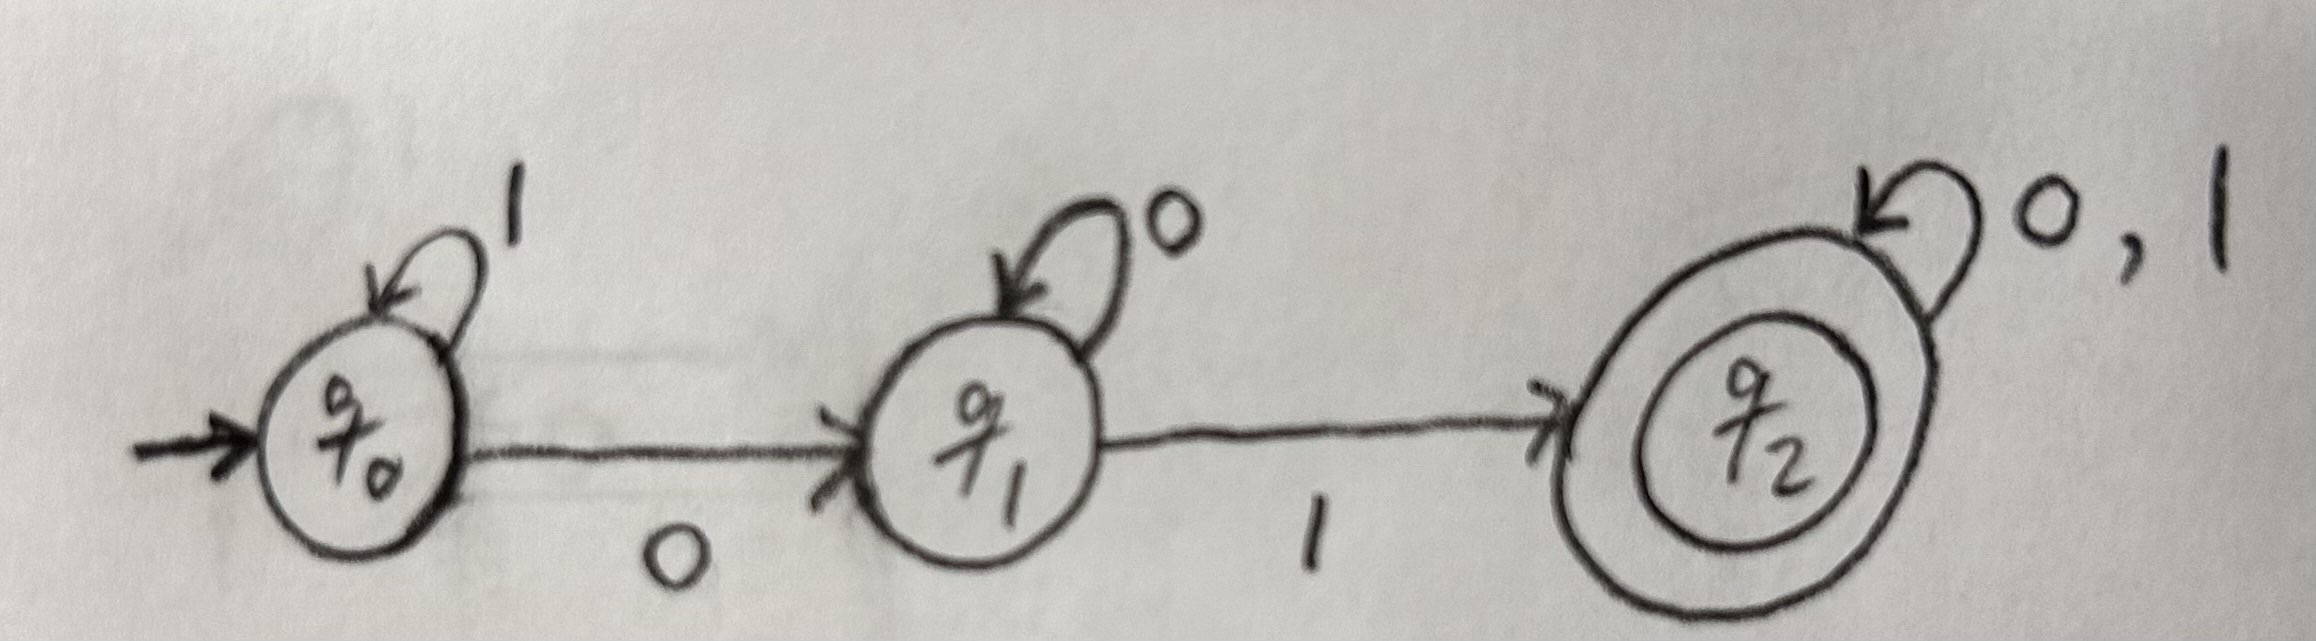
\includegraphics[scale=0.1]{9.3}
          \begin{proof}
              This statement is proven by mutual induction using the following 3 predicates:\\
              $$
                  \begin{aligned}
                       & A(n):=\forall w \in\{0,1\}^* .|w|=n \rightarrow\left(\hat{\delta}\left(q_0, w\right)=q_0 \leftrightarrow w \text { doesn't have 01 as a substring} \right. \\
                       & \quad \left. \text{and doesn't end with } 0\right)                                                                                                         \\
                       & B(n):=\forall w \in\{0,1\}^* .|w|=n \rightarrow\left(\hat{\delta}\left(q_0, w\right)=q_1 \leftrightarrow w \text { doesn't have 01 as a substring} \right. \\
                       & \quad \left. \text{and ends with } 0\right)                                                                                                                \\
                       & C(n):=\forall w \in\{0,1\}^* .|w|=n \rightarrow\left(\hat{\delta}\left(q_0, w\right)=q_2 \leftrightarrow w \text { has 01 as a substring }\right)
                  \end{aligned}
              $$

              \textbf{Base case} $n=0$: Let $w$ be an arbitrary string over the alphabet $\{0,1\}$ that is of length 0. Then we know that $w=\lambda$ and $\hat{\delta}\left(q_0, w\right)=\hat{\delta}\left(q_0, \lambda\right)$. By definition of $\hat{\delta}$, we find that $\hat{\delta}\left(q_0, \lambda\right)=q_0$.\\
              Thus, both sides of $A(0)$'s biconditional are satisfied, rendering $A(0)$ true.\\
              At the same time, since $q_0 \neq q_1, q_0 \neq q_2, \lambda$ does not end with 0, and $\lambda$ does not have 01 as a substring, both sides of $B(0)$'s biconditional are false and both sides of $C(0)$'s biconditional are false, rendering $B(0)$ and $C(0)$ true.\\

              \textbf{Inductive case :} Suppose for the inductive hypothesis that all of $A(n), B(n)$, and $C(n)$ hold for some natural $n$. We want to show each of $A(n+1), B(n+1)$, and $C(n+1)$.\\
              Let $w$ be an arbitrary string over the alphabet $\{0,1\}$ of length $n+1$. Because $n+1 \geq 1$, it must be that $w=v c$ for some string $v \in\{0,1\}^*$ of length $n$ and $c \in\{0,1\}$.\\
              The proof now proceeds by cases over the result of $\hat{\delta}\left(q_0, v\right)$ and the identity of $c$.\\

              \textbf{Subcase }$\hat{\delta}\left(q_0, v\right)=q_0$ and $c=0$: Suppose that $\hat{\delta}\left(q_0, v\right)=q_0$ and $c=0$. Observe then the following:
              $$
                  \begin{aligned}
                      \hat{\delta}\left(q_0, w\right) & =\hat{\delta}\left(q_0, v 0\right)                     & {[w=v c, c=0] }                                     \\
                                                      & =\delta\left(\hat{\delta}\left(q_0, v\right), 0\right) & {[\hat{\delta} \text { def}] }                      \\
                                                      & =\delta\left(q_0, 0\right)                             & {\left[\hat{\delta}\left(q_0, v\right)=q_0\right] } \\
                                                      & =q_1                                                   & {[\delta \operatorname{def}] . }
                  \end{aligned}
              $$
              Further, because $\hat{\delta}\left(q_0, v\right)=q_0$, the inductive hypothesis tells us that $v$ does not have 01 as a substring and does not end with 0. Thus, we know that $w=v0$ does not have 01 as a substring and ends with 0.\\
              This leaves both sides of $B(n+1)$'s biconditional true, rendering $B(n+1)$ true.\\
              At the same time, because $\hat{\delta}\left(q_0, w\right)$ is not $q_0$ or $q_2$ and $w$ does not have 01 as a substring and ends with 0, both sides of $A(n+1)$ and $C(n+1)$'s biconditionals are false, rendering both $A(n+1)$ and $C(n+1)$ true.\\

              \textbf{Subcase }$\hat{\delta}\left(q_0, v\right)=q_0$ and $c=1$: Suppose that $\hat{\delta}\left(q_0, v\right)=q_0$ and $c=1$. Observe then the following:
              $$
                  \begin{aligned}
                      \hat{\delta}\left(q_0, w\right) & =\hat{\delta}\left(q_0, v 1\right)                     & {[w=v c, c=1] }                                     \\
                                                      & =\delta\left(\hat{\delta}\left(q_0, v\right), 1\right) & {[\hat{\delta} \text { def}] }                      \\
                                                      & =\delta\left(q_0, 1\right)                             & {\left[\hat{\delta}\left(q_0, v\right)=q_0\right] } \\
                                                      & =q_0                                                   & {[\delta \operatorname{def}] . }
                  \end{aligned}
              $$
              Further, because $\hat{\delta}\left(q_0, v\right)=q_0$, the inductive hypothesis tells us that $v$ does not have 01 as a substring and does not end with 0. Thus, we know that $w=v1$ does not have 01 as a substring and doesn't end with 0.\\
              This leaves both sides of $A(n+1)$'s biconditional true, rendering $A(n+1)$ true.\\
              At the same time, because $\hat{\delta}\left(q_0, w\right)$ is not $q_1$ or $q_2$ and $w$ does not have 01 as a substring and doesn't end with 0, both sides of $B(n+1)$ and $C(n+1)$'s biconditionals are false, rendering both $B(n+1)$ and $C(n+1)$ true.\\

              \textbf{Subcase }$\hat{\delta}\left(q_0, v\right)=q_1$ and $c=0$: Suppose that $\hat{\delta}\left(q_0, v\right)=q_1$ and $c=0$. Observe then the following:
              $$
                  \begin{aligned}
                      \hat{\delta}\left(q_0, w\right) & =\hat{\delta}\left(q_0, v 0\right)                     & {[w=v c, c=0] }                                     \\
                                                      & =\delta\left(\hat{\delta}\left(q_0, v\right), 0\right) & {[\hat{\delta} \text { def}] }                      \\
                                                      & =\delta\left(q_1, 0\right)                             & {\left[\hat{\delta}\left(q_0, v\right)=q_1\right] } \\
                                                      & =q_1                                                   & {[\delta \operatorname{def}] . }
                  \end{aligned}
              $$
              Further, because $\hat{\delta}\left(q_0, v\right)=q_1$, the inductive hypothesis tells us that $v$ does not have 01 as a substring and ends with 0. Thus, we know that $w=v0$ does not have 01 as a substring and ends with 0.\\
              This leaves both sides of $B(n+1)$'s biconditional true, rendering $B(n+1)$ true.\\
              At the same time, because $\hat{\delta}\left(q_0, w\right)$ is not $q_0$ or $q_2$ and $w$ does not have 01 as a substring and ends with 0, both sides of $A(n+1)$ and $C(n+1)$'s biconditionals are false, rendering both $A(n+1)$ and $C(n+1)$ true.\\

              \textbf{Subcase }$\hat{\delta}\left(q_0, v\right)=q_1$ and $c=1$: Suppose that $\hat{\delta}\left(q_0, v\right)=q_1$ and $c=1$. Observe then the following:
              $$
                  \begin{aligned}
                      \hat{\delta}\left(q_0, w\right) & =\hat{\delta}\left(q_0, v 1\right)                     & {[w=v c, c=1] }                                     \\
                                                      & =\delta\left(\hat{\delta}\left(q_0, v\right), 1\right) & {[\hat{\delta} \text { def}] }                      \\
                                                      & =\delta\left(q_1, 1\right)                             & {\left[\hat{\delta}\left(q_0, v\right)=q_1\right] } \\
                                                      & =q_2                                                   & {[\delta \operatorname{def}] . }
                  \end{aligned}
              $$
              Further, because $\hat{\delta}\left(q_0, v\right)=q_1$, the inductive hypothesis tells us that $v$ does not have 01 as a substring and ends with 0. Thus, we know that $w=v1$ has 01 as a substring.\\
              This leaves both sides of $C(n+1)$'s biconditional true, rendering $C(n+1)$ true.\\
              At the same time, because $\hat{\delta}\left(q_0, w\right)$ is not $q_0$ or $q_1$ and $w$ has 01 as a substring, both sides of $A(n+1)$ and $B(n+1)$'s biconditionals are false, rendering both $A(n+1)$ and $B(n+1)$ true.\\

              \textbf{Subcase }$\hat{\delta}\left(q_0, v\right)=q_2$ and $c=0$: Suppose that $\hat{\delta}\left(q_0, v\right)=q_2$ and $c=0$. Observe then the following:
              $$
                  \begin{aligned}
                      \hat{\delta}\left(q_0, w\right) & =\hat{\delta}\left(q_0, v 0\right)                     & {[w=v c, c=0] }                                     \\
                                                      & =\delta\left(\hat{\delta}\left(q_0, v\right), 0\right) & {[\hat{\delta} \text { def}] }                      \\
                                                      & =\delta\left(q_2, 0\right)                             & {\left[\hat{\delta}\left(q_0, v\right)=q_2\right] } \\
                                                      & =q_2                                                   & {[\delta \operatorname{def}] . }
                  \end{aligned}
              $$
              Further, because $\hat{\delta}\left(q_0, v\right)=q_2$, the inductive hypothesis tells us that $v$ has 01 as a substring. Thus, we know that $w=v0$ has 01 as a substring.\\
              This leaves both sides of $C(n+1)$'s biconditional true, rendering $C(n+1)$ true.\\
              At the same time, because $\hat{\delta}\left(q_0, w\right)$ is not $q_0$ or $q_1$ and $w$ has 01 as a substring, both sides of $A(n+1)$ and $B(n+1)$'s biconditionals are false, rendering both $A(n+1)$ and $B(n+1)$ true.\\

              \textbf{Subcase }$\hat{\delta}\left(q_0, v\right)=q_2$ and $c=1$: Suppose that $\hat{\delta}\left(q_0, v\right)=q_2$ and $c=1$. Observe then the following:
              $$
                  \begin{aligned}
                      \hat{\delta}\left(q_0, w\right) & =\hat{\delta}\left(q_0, v 1\right)                     & {[w=v c, c=1] }                                     \\
                                                      & =\delta\left(\hat{\delta}\left(q_0, v\right), 1\right) & {[\hat{\delta} \text { def}] }                      \\
                                                      & =\delta\left(q_2, 1\right)                             & {\left[\hat{\delta}\left(q_0, v\right)=q_2\right] } \\
                                                      & =q_2                                                   & {[\delta \operatorname{def}] . }
                  \end{aligned}
              $$
              Further, because $\hat{\delta}\left(q_0, v\right)=q_2$, the inductive hypothesis tells us that $v$ has 01 as a substring. Thus, we know that $w=v1$ has 01 as a substring.\\
              This leaves both sides of $C(n+1)$'s biconditional true, rendering $C(n+1)$ true.\\
              At the same time, because $\hat{\delta}\left(q_0, w\right)$ is not $q_0$ or $q_1$ and $w$ has 01 as a substring, both sides of $A(n+1)$ and $B(n+1)$'s biconditionals are false, rendering both $A(n+1)$ and $B(n+1)$ true.\\
              \textbf{Conclusion :} Thus, by mutual induction, $A(n)$, $B(n)$, and $C(n)$ hold for all naturals $n$.\\
              Now observe that the following identities hold for the language of the automaton $M$:
              $$
                  \begin{aligned}
                      \mathcal{L}(M) & =\left\{w \in\{0, 1\}^* \mid \hat{\delta}(q_0, w) \in\{q_2\}\right\}   &  & {[\mathcal{L} \text { def }] } \\
                                     & =\left\{w \in\{0, 1\}^* \mid \hat{\delta}(q_0, w)=q_2\right\}          &  & {[\text { logic }] }           \\
                                     & =\left\{w \in\{0, 1\}^* \mid w \text { has 01 as a substring }\right\} &  & {[C(|w|)] }
                  \end{aligned}
              $$

              This confirms the desired identity for the language of $M$.

          \end{proof}

          \newpage

          9.12 $\left\{w \in\{0,1\}^*: w\right.$ has exactly one 0$\}$\\
          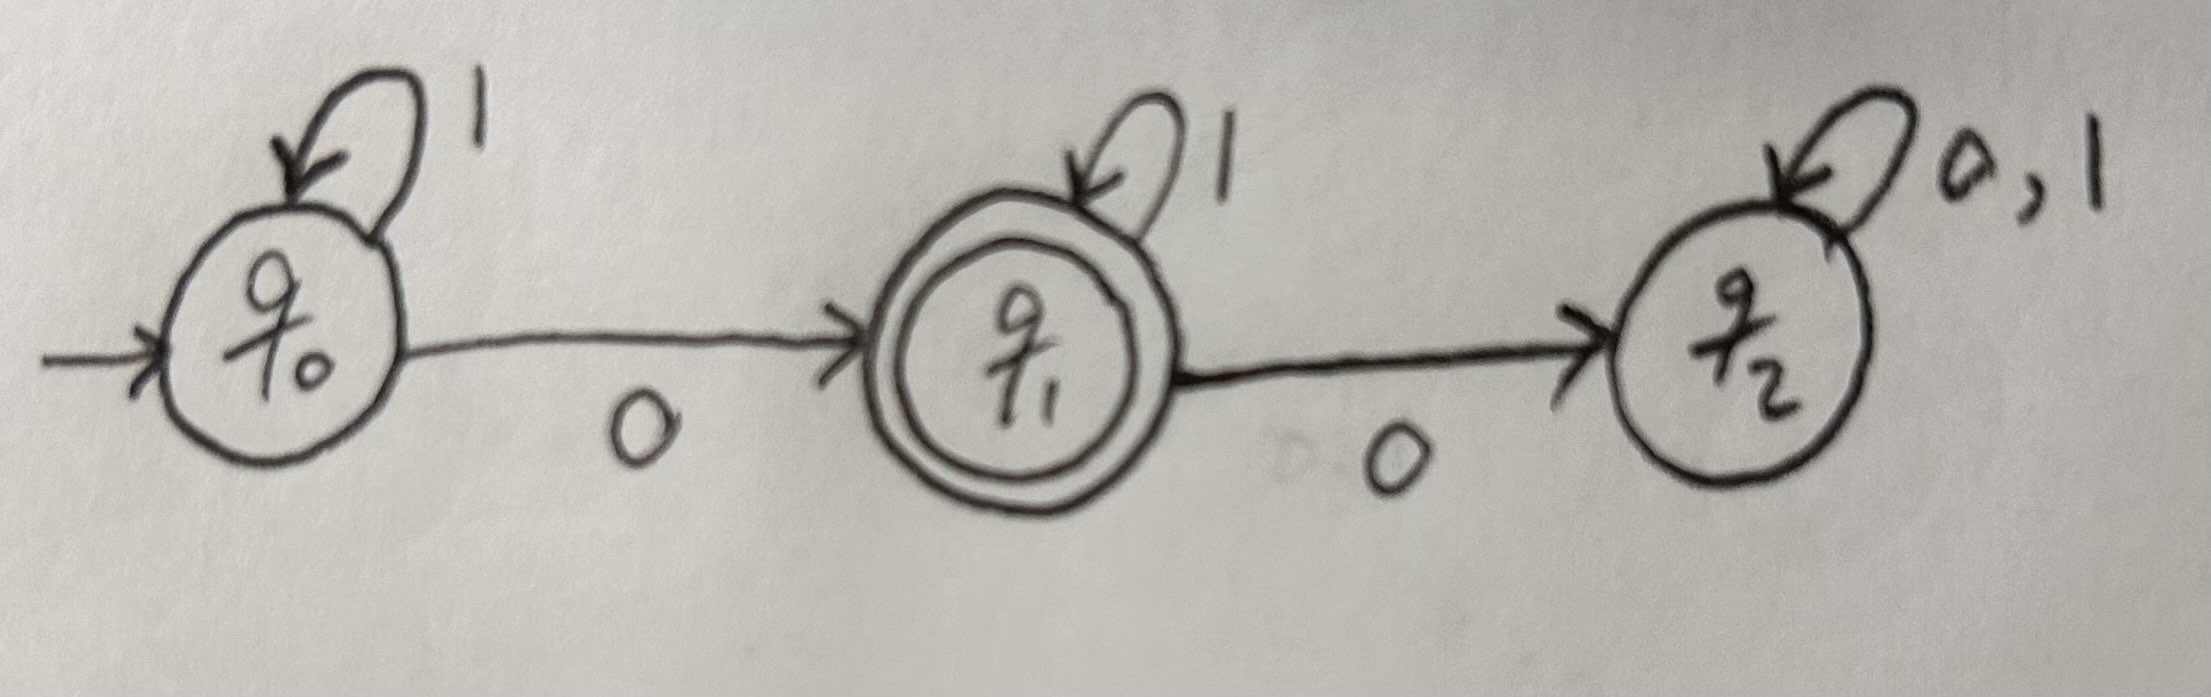
\includegraphics[scale=0.1]{9.12}
          \begin{proof}
              This statement is proven by mutual induction using the following 3 predicates:\\
              $$
                  \begin{aligned}
                       & A(n):=\forall w \in\{0,1\}^* .|w|=n \rightarrow\left(\hat{\delta}\left(q_0, w\right)=q_0 \leftrightarrow w \text { has no } 0\right)            \\
                       & B(n):=\forall w \in\{0,1\}^* .|w|=n \rightarrow\left(\hat{\delta}\left(q_0, w\right)=q_1 \leftrightarrow w \text { has exactly one } 0\right)   \\
                       & C(n):=\forall w \in\{0,1\}^* .|w|=n \rightarrow\left(\hat{\delta}\left(q_0, w\right)=q_2 \leftrightarrow w \text { has at least two 0s }\right)
                  \end{aligned}
              $$

              \textbf{Base case} $n=0$: Let $w$ be an arbitrary string over the alphabet $\{0,1\}$ that is of length 0. Then we know that $w=\lambda$ and $\hat{\delta}\left(q_0, w\right)=\hat{\delta}\left(q_0, \lambda\right)$. By definition of $\hat{\delta}$, we find that $\hat{\delta}\left(q_0, \lambda\right)=q_0$.\\
              Thus, both sides of $A(0)$'s biconditional are satisfied, rendering $A(0)$ true.\\
              At the same time, since $q_0 \neq q_1, q_0 \neq q_2, \lambda$ does not have exactly one 0, and $\lambda$ does not have at least two 0s, both sides of $B(0)$'s biconditional are false and both sides of $C(0)$'s biconditional are false, rendering $B(0)$ and $C(0)$ true.\\

              \textbf{Inductive case :} Suppose for the inductive hypothesis that all of $A(n), B(n)$, and $C(n)$ hold for some natural $n$. We want to show each of $A(n+1), B(n+1)$, and $C(n+1)$.\\
              Let $w$ be an arbitrary string over the alphabet $\{0,1\}$ of length $n+1$. Because $n+1 \geq 1$, it must be that $w=v c$ for some string $v \in\{0,1\}^*$ of length $n$ and $c \in\{0,1\}$.\\
              The proof now proceeds by cases over the result of $\hat{\delta}\left(q_0, v\right)$ and the identity of $c$.\\

              \textbf{Subcase }$\hat{\delta}\left(q_0, v\right)=q_0$ and $c=0$: Suppose that $\hat{\delta}\left(q_0, v\right)=q_0$ and $c=0$. Observe then the following:
              $$
                  \begin{aligned}
                      \hat{\delta}\left(q_0, w\right) & =\hat{\delta}\left(q_0, v 0\right)                     & {[w=v c, c=0] }                                     \\
                                                      & =\delta\left(\hat{\delta}\left(q_0, v\right), 0\right) & {[\hat{\delta} \text { def}] }                      \\
                                                      & =\delta\left(q_0, 0\right)                             & {\left[\hat{\delta}\left(q_0, v\right)=q_0\right] } \\
                                                      & =q_1                                                   & {[\delta \operatorname{def}] . }
                  \end{aligned}
              $$
              Further, because $\hat{\delta}\left(q_0, v\right)=q_0$, the inductive hypothesis tells us that $v$ has no 0. Thus, we know that $w=v0$ has exactly one 0.\\
              This leaves both sides of $B(n+1)$'s biconditional true, rendering $B(n+1)$ true.\\
              At the same time, because $\hat{\delta}\left(q_0, w\right)$ is not $q_0$ or $q_2$ and $w$ has exactly one 0, both sides of $A(n+1)$ and $C(n+1)$'s biconditionals are false, rendering both $A(n+1)$ and $C(n+1)$ true.\\

              \textbf{Subcase }$\hat{\delta}\left(q_0, v\right)=q_0$ and $c=1$: Suppose that $\hat{\delta}\left(q_0, v\right)=q_0$ and $c=1$. Observe then the following:
              $$
                  \begin{aligned}
                      \hat{\delta}\left(q_0, w\right) & =\hat{\delta}\left(q_0, v 1\right)                     & {[w=v c, c=1] }                                     \\
                                                      & =\delta\left(\hat{\delta}\left(q_0, v\right), 1\right) & {[\hat{\delta} \text { def}] }                      \\
                                                      & =\delta\left(q_0, 1\right)                             & {\left[\hat{\delta}\left(q_0, v\right)=q_0\right] } \\
                                                      & =q_0                                                   & {[\delta \operatorname{def}] . }
                  \end{aligned}
              $$
              Further, because $\hat{\delta}\left(q_0, v\right)=q_0$, the inductive hypothesis tells us that $v$ has no 0. Thus, we know that $w=v1$ has no 0.\\
              This leaves both sides of $A(n+1)$'s biconditional true, rendering $A(n+1)$ true.\\
              At the same time, because $\hat{\delta}\left(q_0, w\right)$ is not $q_1$ or $q_2$ and $w$ has no 0, both sides of $B(n+1)$ and $C(n+1)$'s biconditionals are false, rendering both $B(n+1)$ and $C(n+1)$ true.\\

              \textbf{Subcase }$\hat{\delta}\left(q_0, v\right)=q_1$ and $c=0$: Suppose that $\hat{\delta}\left(q_0, v\right)=q_1$ and $c=0$. Observe then the following:
              $$
                  \begin{aligned}
                      \hat{\delta}\left(q_0, w\right) & =\hat{\delta}\left(q_0, v 0\right)                    & {[w=v c, c=0] }                                     \\
                                                      & =\delta\left(\hat{\delta}\left(q_0, v\right),0\right) & {[\hat{\delta} \text { def}] }                      \\
                                                      & =\delta\left(q_1, 0\right)                            & {\left[\hat{\delta}\left(q_0, v\right)=q_1\right] } \\
                                                      & =q_2                                                  & {[\delta \operatorname{def}] . }
                  \end{aligned}
              $$
              Further, because $\hat{\delta}\left(q_0, v\right)=q_1$, the inductive hypothesis tells us that $v$ has exactly one 0. Thus, we know that $w=v0$ has at least two 0s.\\
              This leaves both sides of $C(n+1)$'s biconditional true, rendering $C(n+1)$ true.\\
              At the same time, because $\hat{\delta}\left(q_0, w\right)$ is not $q_0$ or $q_1$ and $w$ has at least two 0s, both sides of $A(n+1)$ and $B(n+1)$'s biconditionals are false, rendering both $A(n+1)$ and $B(n+1)$ true.\\

              \textbf{Subcase }$\hat{\delta}\left(q_0, v\right)=q_1$ and $c=1$: Suppose that $\hat{\delta}\left(q_0, v\right)=q_1$ and $c=1$. Observe then the following:
              $$
                  \begin{aligned}
                      \hat{\delta}\left(q_0, w\right) & =\hat{\delta}\left(q_0, v 1\right)                    & {[w=v c, c=1] }                                     \\
                                                      & =\delta\left(\hat{\delta}\left(q_0, v\right),1\right) & {[\hat{\delta} \text { def}] }                      \\
                                                      & =\delta\left(q_1, 1\right)                            & {\left[\hat{\delta}\left(q_0, v\right)=q_1\right] } \\
                                                      & =q_1                                                  & {[\delta \operatorname{def}] . }
                  \end{aligned}
              $$
              Further, because $\hat{\delta}\left(q_0, v\right)=q_1$, the inductive hypothesis tells us that $v$ has exactly one 0. Thus, we know that $w=v1$ has exactly one 0.\\
              This leaves both sides of $B(n+1)$'s biconditional true, rendering $B(n+1)$ true.\\
              At the same time, because $\hat{\delta}\left(q_0, w\right)$ is not $q_0$ or $q_2$ and $w$ has exactly one 0, both sides of $A(n+1)$ and $C(n+1)$'s biconditionals are false, rendering both $A(n+1)$ and $C(n+1)$ true.\\

              \textbf{Subcase }$\hat{\delta}\left(q_0, v\right)=q_2$ and $c=0$: Suppose that $\hat{\delta}\left(q_0, v\right)=q_2$ and $c=0$. Observe then the following:
              $$
                  \begin{aligned}
                      \hat{\delta}\left(q_0, w\right) & =\hat{\delta}\left(q_0, v 0\right)                    & {[w=v c, c=0] }                                     \\
                                                      & =\delta\left(\hat{\delta}\left(q_0, v\right),0\right) & {[\hat{\delta} \text { def}] }                      \\
                                                      & =\delta\left(q_2, 0\right)                            & {\left[\hat{\delta}\left(q_0, v\right)=q_2\right] } \\
                                                      & =q_2                                                  & {[\delta \operatorname{def}] . }
                  \end{aligned}
              $$
              Further, because $\hat{\delta}\left(q_0, v\right)=q_2$, the inductive hypothesis tells us that $v$ has at least two 0s. Thus, we know that $w=v0$ has at least two 0s.\\
              This leaves both sides of $C(n+1)$'s biconditional true, rendering $C(n+1)$ true.\\
              At the same time, because $\hat{\delta}\left(q_0, w\right)$ is not $q_0$ or $q_1$ and $w$ has at least two 0s, both sides of $A(n+1)$ and $B(n+1)$'s biconditionals are false, rendering both $A(n+1)$ and $B(n+1)$ true.\\

              \textbf{Subcase }$\hat{\delta}\left(q_0, v\right)=q_2$ and $c=1$: Suppose that $\hat{\delta}\left(q_0, v\right)=q_2$ and $c=1$. Observe then the following:
              $$
                  \begin{aligned}
                      \hat{\delta}\left(q_0, w\right) & =\hat{\delta}\left(q_0, v 1\right)                    & {[w=v c, c=1] }                                     \\
                                                      & =\delta\left(\hat{\delta}\left(q_0, v\right),1\right) & {[\hat{\delta} \text { def}] }                      \\
                                                      & =\delta\left(q_2, 1\right)                            & {\left[\hat{\delta}\left(q_0, v\right)=q_2\right] } \\
                                                      & =q_2                                                  & {[\delta \operatorname{def}] . }
                  \end{aligned}
              $$
              Further, because $\hat{\delta}\left(q_0, v\right)=q_2$, the inductive hypothesis tells us that $v$ has at least two 0s. Thus, we know that $w=v1$ has at least two 0s.\\
              This leaves both sides of $C(n+1)$'s biconditional true, rendering $C(n+1)$ true.\\
              At the same time, because $\hat{\delta}\left(q_0, w\right)$ is not $q_0$ or $q_1$ and $w$ has at least two 0s, both sides of $A(n+1)$ and $B(n+1)$'s biconditionals are false, rendering both $A(n+1)$ and $B(n+1)$ true.\\

              \textbf{Conclusion :} Thus, by mutual induction, $A(n)$, $B(n)$, and $C(n)$ hold for all naturals $n$.\\
              Now observe that the following identities hold for the language of the automaton $M$:
              $$
                  \begin{aligned}
                      \mathcal{L}(M) & =\left\{w \in\{0, 1\}^* \mid \hat{\delta}(q_0, w) \in\{q_1\}\right\} &  & {[\mathcal{L} \text { def }] } \\
                                     & =\left\{w \in\{0, 1\}^* \mid \hat{\delta}(q_0, w)=q_1\right\}        &  & {[\text { logic }] }           \\
                                     & =\left\{w \in\{0, 1\}^* \mid w \text { has exactly one 0 }\right\}   &  & {[B(|w|)] }
                  \end{aligned}
              $$

              This confirms the desired identity for the language of $M$.
          \end{proof}

\end{enumerate}


\end{document}